\documentclass{article}
\RequirePackage{amssymb}
\RequirePackage{amsmath}
\usepackage{graphicx}
\usepackage[latin1]{inputenc}

\title{Esercizio 6}
\author{Davide Angelocola}

\begin{document}
\maketitle

\section{Esercizio}
Tre libri sono messi uno sopra l'altro a formare una pila. In ogni istante se ne sceglie a caso uno e si mette in cima alla pila lasciando invariata la posizione degli altri due. Assumendo che i libri siano contraddistinti con le lettere A, B e C: descrivere con una catena di Markov il sistema il stato � costituito in ogni istante dalla disposizione dei libri nella pila.

\section{Svolgimento}

Assumendo che la pila di libri sia inizialmente cos� composta:

$$S_1 = \begin{pmatrix} 
A \cr 
B \cr
C \cr 
\end{pmatrix}$$

Prendendo in fondo e ponendolo in cima alla pila, ovvero prendendo il libro C e mettendolo sopra A, si ottiene la seguente pila:

$$S_2 = \begin{pmatrix} 
C \cr 
A \cr
B \cr 
\end{pmatrix}$$

Pescando invece il libro B si ottiene una terza pila:

$$S_3 = \begin{pmatrix} 
B \cr 
A \cr 
C \cr
\end{pmatrix}$$

Risulta quindi si hanno $3!$ possibili configurazioni delle pile, ovvero in quanti modi possiamo disporre $3$ oggetti. Le altre tre configurazioni sono:

$$
S_4 = \begin{pmatrix} 
B \cr 
C \cr 
A \cr
\end{pmatrix}
S_5 = \begin{pmatrix} 
B \cr 
C \cr 
A \cr
\end{pmatrix}
S_6 = \begin{pmatrix} 
B \cr 
C \cr 
A \cr
\end{pmatrix}
$$

Risulta quindi il seguente grafo:

\begin{figure}[t]
\centering
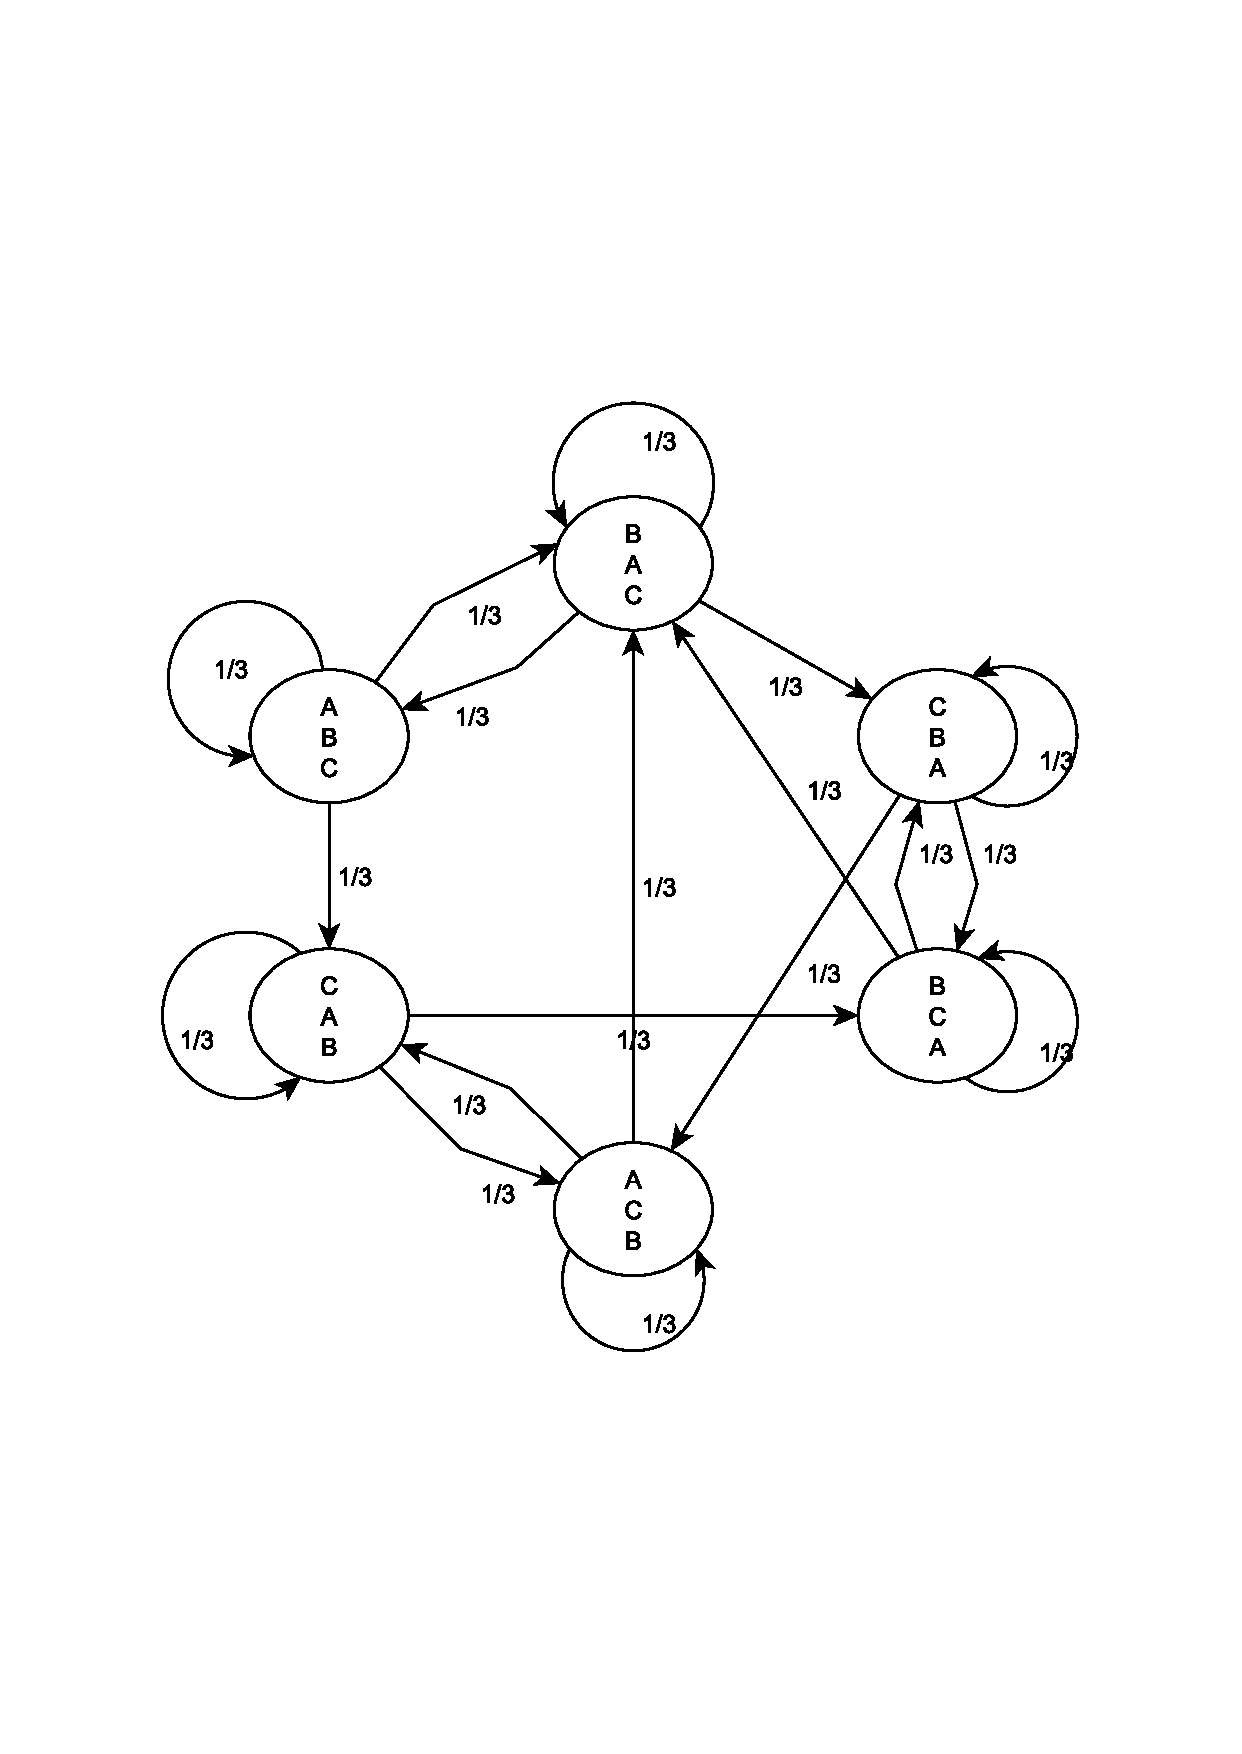
\includegraphics[scale=0.70]{cp_ex6_fig1.pdf}
\caption{Grafo delle transizioni}
\label{fig:}
\end{figure}

\end{document}
